\documentclass{beamer}
\beamertemplatenavigationsymbolsempty
\usecolortheme{beaver}
\setbeamertemplate{blocks}[rounded=true, shadow=true]
\setbeamertemplate{footline}[page number]
%
\usepackage[utf8]{inputenc}
\usepackage[english,russian]{babel}
\usepackage{amssymb,amsfonts,amsmath,mathtext}
\usepackage{subfig}
\usepackage[all]{xy} % xy package for diagrams
\usepackage{array}
\usepackage{multicol}% many columns in slide
\usepackage{hyperref}% urls
\usepackage{hhline}%tables
\usepackage{graphicx}

% Your figures are here:
\graphicspath{ {fig/} {../fig/} }

%----------------------------------------------------------------------------------------------------------
\title{Поиск границ радужки\\ методом круговых проекций}
\author[А.\,А. Баженов]{Баженов Андрей Александрович}
\institute{Московский физико-технический институт}
\date{\footnotesize
\par\smallskip\emph{Курс:} Автоматизация научных исследований\par (практика, В.\,В.~Стрижов)/Группа 821
\par\smallskip\emph{Эксперт:} И.\,А.~Матвеев
\par\smallskip\emph{Консультант:} И.\,А.~Матвеев
\par\bigskip\small 2021}
%----------------------------------------------------------------------------------------------------------
\begin{document}
%----------------------------------------------------------------------------------------------------------
\begin{frame}
\thispagestyle{empty}
\maketitle
\end{frame}

\begin{frame}{Цели исследования}
\begin{block}{Цель исследования}
Исследовать возможность применения метода круговых проекций яркости в качестве метода понижения размерности в задачах машинного обучения.
\end{block}
\begin{block}{Задача}
Построить алгоритм нахождения приблизительных границ элементов глаза на чёрно-белых фотографиях. 
\end{block}
\end{frame}

\begin{frame}{Круговые проекции яркости}
\begin{columns}[c]
\column{0.5\textwidth}
		$\vec{x}$~--- точка изображения\\ 
		$\vec{g}(\vec{x})$~--- градиент яркости\\
		$v_U(\vec{x})$~--- индикатор возможности принадлежности границе\\
		$\Pi_U(r)$~--- усредненное значение индикатора по кругу радиуса $r$
\column{0.5\textwidth}
	\begin{picture}(100,200)
	\put(0, -10){
	  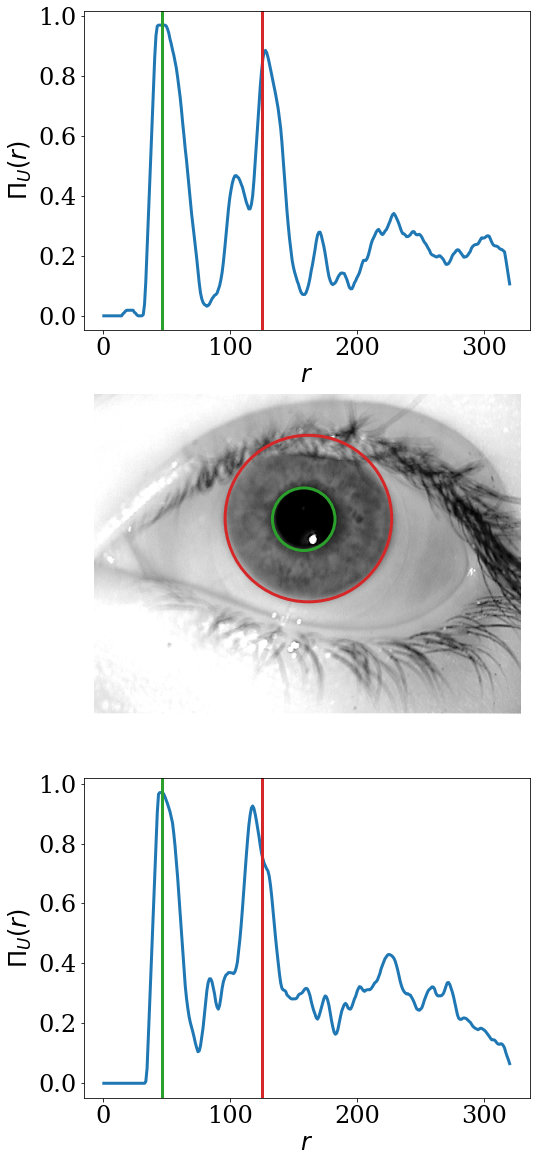
\includegraphics[scale=0.27]{img/eye.png}}
	 \put(64, 160){\vector(-4, -1){15}}
	 \put(45, 147){$\vec{g}(\vec{x})$}
    \end{picture}
\end{columns}

\end{frame}
\begin{frame}{Литература}

\begin{enumerate}
	\item Обзор алгоритмов обнаружения радужки
	
	A.~Nithya and C.~Lakshmi. Iris Recognition Techniques: A Literature Survey. 2015
	
	K.~Bowyer, K.~Hollingsworth, and P.~Flynn. Image Understanding for Iris Biometrics: A Survey. 2008
	
	\item Описание метода круговых проекций
	
	I.\,A.~Matveev. Detection of iris in image by interrelated maxima of brightness gradient projections. 2010
	
\end{enumerate}
\end{frame}

\begin{frame}{Постановка задачи}

\begin{block}{Дано}
Выборка $\mathcal{M} = \left\{\left(M(i), P_\text{R}(i), I_\text{R}(i)\right)\right\}_{i=1}^n$~--- множество растровых изображений со зрачком радиуса $P_\text{R}$ и радужкой радиуса $I_\text{R}$.
\end{block} 

\begin{block}{Требуется}
Построить алгоритм
\[
	f\!: \quad M \mapsto \left(P_\text{R}, I_\text{R}\right).
\]
\end{block}

\begin{block}{Модель}
Рассматриваются алгоритмы вида
\[
f = g \circ \Pi,
\]
$\Pi$~--- процедура подсчета круговых проекций,
\[
g(x) = \sigma_k\left(W_k^T \sigma_{k-1}\left(\ldots \sigma_1\left(W_1^T x\right)\ldots\right)\right).
\] 
\end{block}

\end{frame}

\begin{frame}{Критерий качества}

Пусть $\left(\widehat{P}_\text{R}(i), \widehat{I}_\text{R}(i)\right) = f(M(i))$. Рассматривается $L$~--- кусочно линейное преобразование относительной ошибки.

\begin{block}{Задача оптимизации}
\[
f_0 = \arg\min_{f \in \mathcal{F}} \sum_{i=1}^n L\left(\widehat{P}_\text{R}(i), P_\text{R}(i)\right) + L\left(\widehat{I}_\text{R}(i), I_\text{R}(i)\right).
\]
\end{block}

\end{frame}

\begin{frame}{Обработка круговых проекций}

\begin{block}{Гипотеза}

Значения $P_\text{R}$ и $I_\text{R}$ являются точками локальных максимумов функции $\Pi_U(r)$.

\end{block}

Для выделения максимумов и их обработки используются линенйные, сверточные и реккурентные нейронные сети, обучаемые по метрике MSE.

\end{frame}

\begin{frame}{Результаты эксперимента}

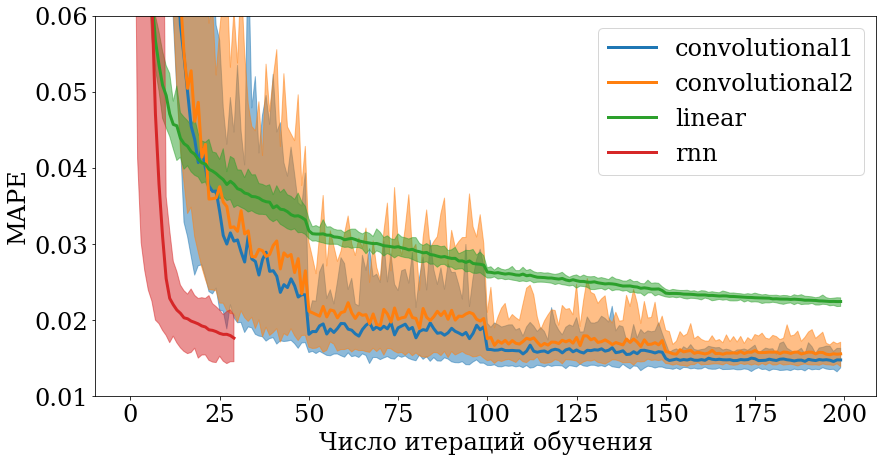
\includegraphics[scale=0.35]{img/mape.png}

\end{frame}

\begin{frame}{Результаты эксперимента}

\begin{center}

\begin{tabular}{|m{2.2cm}|m{1.9cm}|m{3cm}|m{1.9cm}|}

\hline

& Среднее значение ошибки, \% & Доверительный интервал ошибки & Число параметров\\
\hline

Сверточная сеть & $1.39$ & $1.32$-$1.47$ & $56831$\\
\hline
Сверточная сеть & $1.48$ & $1.39$-$1.58$ & $17655$\\
\hline
Линейная сеть & $2.21$ & $2.15$-$2.24$ & $166402$\\
\hline
Реккурентная сеть & $1.77$ & $1.45$-$2.05$ & $14962$\\
\hline
\end{tabular}

\end{center}

\end{frame}

\end{document}